% =============================================================================
% Part II, Chapter 8: Cohorts 013--017
% =============================================================================
\chapter{Two-Study Evidence Selection, the Prospective Order Confirmation, and the Retrospective Shortcut Counterexample (Cohorts 013--017)}\label{ch:cohorts_013_017}

Chapters~5--7 showed how disciplined reference gating prevented premature quantization claims across twelve consecutive cohorts. In Cohorts~013--017 (November 12--13, 2026), CausalFade experienced its most dramatic emotional and scientific arc: solving strict bare-JSON compliance (Cohorts~013--014), passing a 7B \texttt{F16} reference gate for the first time (Cohort~015), prospectively confirming an extraordinary $+62.5\pp$ ($p = 1.24\times 10^{-37}$) quantized evidence-order crossover across $96$ fresh families in Cohort~016, watching that pattern vanish at $14\text{B}$ in Cohort~017, and later discovering during retrospective benchmark auditing that Cohort~016's entire task family admitted a $100\%$-accurate ($768/768$) source-blind numerical magnitude shortcut (Figure~\ref{fig:shortcut_c16}).

\begin{figure}[htbp]
  \centering
  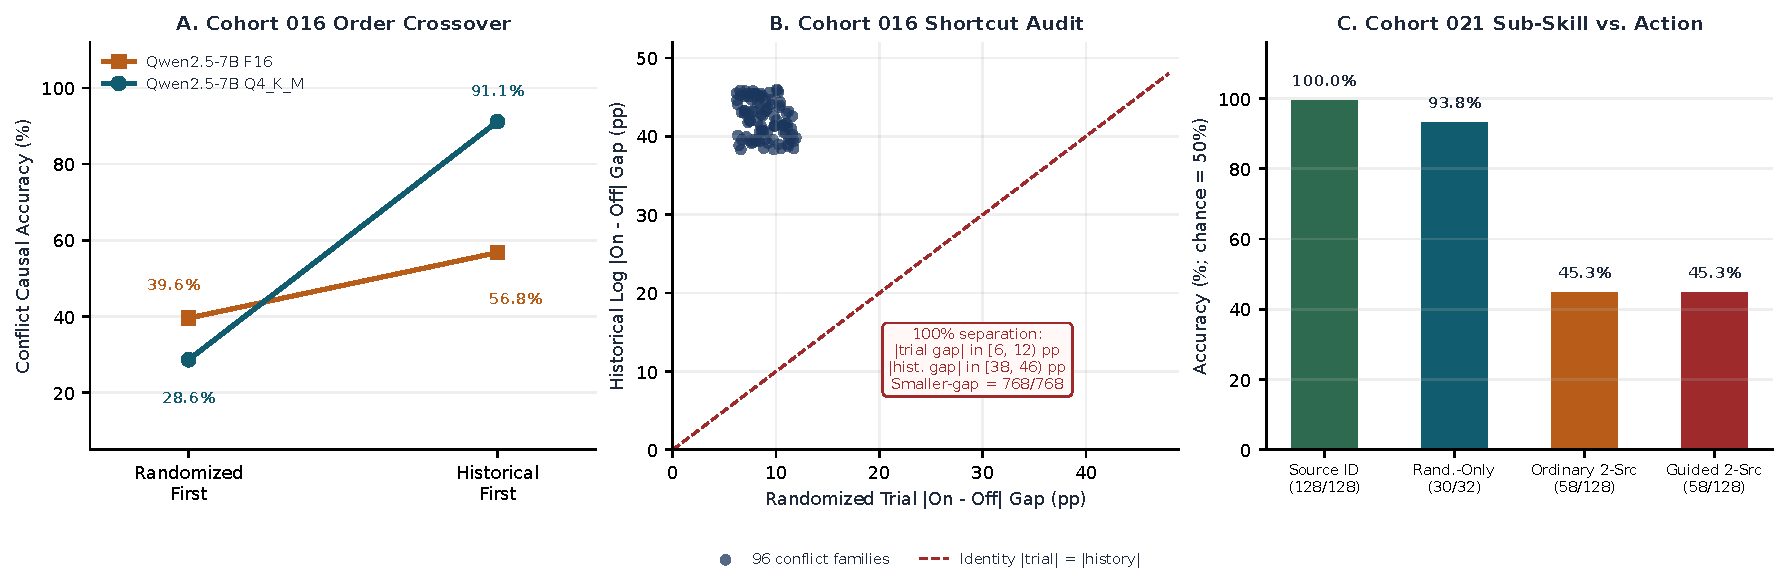
\includegraphics[width=\textwidth]{figures/fig09_evidence_selection_and_shortcut.pdf}
  \caption{The Cohort~016 order confirmation, its retrospective shortcut counterexample, and Cohort~021's component dissociation: (A) Cohort~016 96-family conflict accuracy by presentation order for \texttt{Qwen2.5-7B F16} and \texttt{Q4\_K\_M}; (B) Retrospective source-blind separation showing $|\text{trial gap}| \in [6,12)\pp < |\text{history gap}| \in [38,46)\pp$ on $100\%$ of items; (C) Cohort~021 governing-source recognition ($100\%$) vs.\ two-source decision failure ($45.3\%$).}
  \label{fig:shortcut_c16}
\end{figure}

% =============================================================================
\section{Cohort 013: Minimal vs.\ Causal-Context Prompt Crossover (160-Token Post-JSON Verbosity Failure)}

\subsection*{1. Historical Context}
Cohort~012 failed because minimal study labels (\emph{``Historical data where operators chose...''}) did not cue \texttt{Qwen2.5-7B F16} to discount confounding. Cohort~013 crossed that minimal prompt against a richer \emph{causal-context} prompt explicitly explaining that unmeasured initial severity affects both historical operator choices and outcomes.

\subsection*{2. Research Question}
Does adding explicit causal-confounding context allow \texttt{Qwen2.5-7B F16} to pass the two-study conflict reference gate?

\subsection*{3. Hypothesis}
\textbf{Classification:} \emph{Exploratory prompt-clarity crossover.} Expected causal-context prose to raise conflict accuracy above $\ge 9/16$ per order.

\subsection*{4. Experimental Design}
Single model (\texttt{Qwen2.5-7B F16}) on $8$ fresh matched-strength families (\texttt{seed=20261116}) $\times 4$ cells $\times 2$ orders $\times 2$ prompt frames (\texttt{minimal} vs.\ \texttt{causal\_context}) $= 128$ prompts (\texttt{max\_tokens=160}).

\subsection*{5. Mathematical Formulation}
Identical matched-strength two-study causal contrast (\texttt{M06}), paired within family across prompt frames.

\subsection*{6. Experimental Execution}
Completed November 12, 2026 (commit \texttt{0f55a79}). An unexpected formatting failure occurred on $64/64$ causal-context items!

\subsection*{7. Results}
\begin{itemize}
  \item \textbf{Minimal Frame:} $64/64$ single-fence valid ($0/64$ bare JSON); scored \textbf{$48/64$ ($75.0\%$)\textbf{ overall ($32/32$ aligned, }$8/16$} and \textbf{$8/16$} conflict---again failing the $\ge 9/16$ conflict gate).
  \item \textbf{Causal-Context Frame:} \textbf{$0/64$ valid} under both strict bare JSON \emph{and} single-fence parsing! Because the prompt mentioned causal reasoning concepts, \texttt{Qwen2.5-7B F16} emitted a valid fenced JSON object first and then \emph{appended a multi-sentence causal explanation afterward}, running straight into the $160$-token cap on all $64$ items! A post-hoc prefix diagnostic extracting the leading JSON scored $45/64$, which was properly refused for gate qualification.
\end{itemize}

\subsection*{8. Interpretation at the Time}
Prompting LLMs about confounding triggers didactic post-JSON explanations unless the output contract explicitly forbids Markdown fences and trailing text.

\subsection*{9. Retrospective Interpretation}
This failure directly catalyzed CausalFade's transition to strict bare-JSON contracts (\emph{``Do not include a Markdown fence, explanation, or any other text''}), raising strict bare-JSON validity from $0\%$ (Cohorts~001--013) to \textbf{$100\%$} across Cohorts~014--023 and 029!

\subsection*{10. Methodological Limitations}
Post-JSON verbosity invalidated the causal-context arm; 8-family development size.

\subsection*{11. Scientific Contribution}
\emph{Infrastructure discovery:} Identified explanation-triggering prompt spillover and motivated strict bare-JSON negative constraints.

\subsection*{12. Transition to Subsequent Research}
Cohort~014 tightened the output instruction and lowered \texttt{max\_tokens} to $48$ on $8$ fresh families.

\subsection*{13. Evidence and Reproducibility}
Artifacts: \texttt{experiments/cohort\_013/summary.md}, \texttt{run\_001\_7b\_f16/}; commit \texttt{0f55a79}.

% =============================================================================
\section{Cohort 014: Strict Bare-JSON Contract Screen (48-Token Cap)}

\subsection*{1. Historical Context}
Cohort~014 immediately tested a hardened strict-JSON output instruction (\texttt{max\_tokens=48}) across both minimal and causal-context frames on fresh families.

\subsection*{2. Research Question}
Does an explicit bare-JSON anti-fence instruction achieve $\ge 95\%$ strict JSON validity on \texttt{Qwen2.5-7B F16}, and does either frame clear the reference competence gate?

\subsection*{3. Hypothesis}
\textbf{Classification:} \emph{Documented prospective feasibility gate.} Pre-declared gate: strict bare-JSON validity $\ge 56/64$, overall accuracy $\ge 44/64$ ($68.75\%$), and conflict accuracy $\ge 9/16$ in each presentation order.

\subsection*{4. Experimental Design}
\texttt{Qwen2.5-7B F16} on $8$ fresh matched-strength families (\texttt{seed=20261119}), $64$ minimal + $64$ causal-context prompts $= 128$ requests (\texttt{max\_tokens=48}, \texttt{temperature=0.0}).

\subsection*{5. Mathematical Formulation}
Identical matched-strength two-study contrast (\texttt{M06}) scored under exact \texttt{json.loads} without fence stripping.

\subsection*{6. Experimental Execution}
Completed November 12, 2026 (commit \texttt{baa573b}). Verbatim output on every single item: \texttt{\{"activate": 1\}} or \texttt{\{"activate": 0\}}.

\subsection*{7. Results}
\begin{itemize}
  \item \textbf{Strict Bare-JSON Validity Solved:} \textbf{$128/128$ ($100.0\%$)} strict bare-JSON compliance with normal stops!
  \item \textbf{Near-Miss Gate Outcome:}
    \begin{itemize}
      \item \texttt{Minimal}: $48/64$ overall (passed $\ge 44$), $32/32$ aligned, but \textbf{$8/16$} and \textbf{$8/16$} conflict (\textbf{failed} $\ge 9/16$ conflict gate).
      \item \texttt{Causal-context}: \textbf{$9/16$ ($56.25\%$)} randomized-first conflict and \textbf{$9/16$ ($56.25\%$)} historical-first conflict (\textbf{passed} both conflict gates!), plus $24/32$ aligned, totaling \textbf{$42/64$ ($65.63\%$)} overall---missing the $\ge 44/64$ overall threshold by just $2$ items!
    \end{itemize}
\end{itemize}

\subsection*{8. Interpretation at the Time}
Strict bare JSON worked flawlessly ($128/128$), and causal-context framing cleared per-order conflict thresholds for the first time in the project, missing the overall 8-family gate by $2$ items under high discrete binomial noise.

\subsection*{9. Retrospective Interpretation}
Notice a subtle sign of trouble that would soon grow: adding causal context lowered \emph{aligned} accuracy from $32/32$ to $24/32$ ($75\%$), showing that causal-context prose perturbed aligned choices even when both studies agreed!

\subsection*{10. Methodological Limitations}
Underpowered $8$-family ($16$-item per conflict order) discrete threshold; unacknowledged $|\tau| < |\RD_{\mathrm{obs}}|$ gap invariant.

\subsection*{11. Scientific Contribution}
\emph{Infrastructure breakthrough ($100\%$ strict bare-JSON compliance) \& narrow reference-gate diagnostic.}

\subsection*{12. Transition to Subsequent Research}
Cohort~015 doubled the sample size to $16$ fresh families ($128$ causal-context prompts) with scaled pre-declared gate thresholds ($\ge 88/128$ overall, $\ge 18/32$ per conflict order) and conditional authorization to run \texttt{7B Q4\_K\_M} if \texttt{F16} passed.

\subsection*{13. Evidence and Reproducibility}
Artifacts: \texttt{experiments/cohort\_014/summary.md}, \texttt{run\_001\_7b\_f16/}; commit \texttt{baa573b}.

% =============================================================================
\section{Cohort 015: 16-Family Causal-Context Gate Pass and Discovery of the \texttt{7B Q4\_K\_M} Order Jump}

\subsection*{1. Historical Context}
Cohort~015 executed the scaled 16-family causal-context gate on \texttt{Qwen2.5-7B F16}, with a frozen plan (\texttt{frozen\_run\_plan.json}) authorizing \texttt{Qwen2.5-7B Q4\_K\_M} \emph{if and only if} \texttt{F16} cleared every threshold.

\subsection*{2. Research Question}
Does \texttt{Qwen2.5-7B F16} clear the 16-family causal-context competence gate, and if triggered, how does \texttt{7B Q4\_K\_M} compare across aligned, conflict, and study-order conditions?

\subsection*{3. Hypothesis}
\textbf{Classification:} \emph{Documented prospective gate + conditional exploratory format comparison (\texttt{H01}, \texttt{H06}).}

\subsection*{4. Experimental Design}
\texttt{Qwen2.5-7B} \texttt{F16} (\texttt{run\_001\_7b\_f16}) and conditionally triggered \texttt{Q4\_K\_M} (\texttt{run\_002\_7b\_q4\_k\_m}) on $16$ fresh matched-strength families (\texttt{seed=20261122}), $128$ strict-JSON prompts/arm ($256$ total requests).

\subsection*{5. Mathematical Formulation}
Paired 16-family comparisons on overall accuracy, conflict penalty, and within-family order contrast $\Delta_{\mathrm{order}}(p) = \mathrm{Acc}_{\mathrm{conflict}}(\mathrm{hist\text{-}first}, p) - \mathrm{Acc}_{\mathrm{conflict}}(\mathrm{rand\text{-}first}, p)$.

\subsection*{6. Experimental Execution}
Completed November 12, 2026 (commit \texttt{79c0ba5}); $256/256$ strict-valid bare JSON responses.

\subsection*{7. Results}
\emph{(From \texttt{experiments/cohort\_015/summary.md}.)}
\begin{itemize}
  \item \textbf{\texttt{7B F16} Cleared All Gate Thresholds:} $128/128$ valid ($\ge 112$), \textbf{$89/128$ ($69.53\%$)} overall ($\ge 88$), \textbf{$19/32$ ($59.38\%$)} rand-first conflict ($\ge 18$), and \textbf{$22/32$ ($68.75\%$)} hist-first conflict ($\ge 18$), legitimately triggering \texttt{Q4\_K\_M}.
  \item \textbf{\texttt{7B Q4\_K\_M} Scored Higher Overall---With a Massive $+65.6\pp$ Conflict Order Swing:}
    \begin{itemize}
      \item Aggregate \texttt{Q4\_K\_M} scored \textbf{$98/128$ ($76.56\%$)} overall ($+7.03\pp$ above \texttt{F16}, 95\% CI $[+0.78, +12.50]\pp$), with $55/64$ aligned and $43/64$ conflict (conflict-penalty difference $+7.81\pp$, CI $[-7.81, +23.44]\pp$).
      \item Splitting by study order revealed an astonishing pattern: on conflict items, \texttt{Q4\_K\_M} scored \textbf{$11/32$ ($34.38\%$)} when randomized evidence was first vs.\ \textbf{$32/32$ ($100.00\%$)\textbf{ when historical evidence was first (}$+65.625\pp$}, CI $[+56.25, +78.13]\pp$), compared to $+9.375\pp$ on \texttt{F16} (format-by-order interaction \textbf{$+56.25\pp$}, CI $[+40.63, +71.88]\pp$)!
      \item Conversely, on \emph{aligned} items, historical-first \emph{reduced} accuracy from $32/32$ to $16/32$ ($-50.0\pp$) on \texttt{F16} and from $32/32$ to $23/32$ ($-28.1\pp$) on \texttt{Q4\_K\_M}!
    \end{itemize}
\end{itemize}

\subsection*{8. Interpretation at the Time}
The researchers resisted claiming victory from a 16-family exploratory surprise: \texttt{summary.md} explicitly classified Cohort~015 as development data and pre-registered a dedicated $96$-family prospective replication of the \texttt{Q4\_K\_M} conflict-order effect in Cohort~016 (\texttt{D06}).

\subsection*{9. Retrospective Interpretation}
Look at \texttt{Q4\_K\_M}'s conflict split: $32/32$ ($100\%$) when randomized evidence was \emph{second} (historical first), vs.\ $11/32$ ($34.4\%$) when randomized evidence was \emph{first} (historical second). In a two-study prompt where the model strongly weights the \emph{final} numbers right above the question (recency bias \citep{liu2024lost}), placing the randomized trial second puts the right numbers in the recency slot, whereas placing the historical study second puts the misleading confounded numbers in the recency slot!

\subsection*{10. Methodological Limitations}
$16$ development families; single checkpoint lineage; aligned-item order drop ($-50\pp$ in \texttt{F16}) signaled strange prompt-order heuristics; hidden $|\tau| < |\RD_{\mathrm{obs}}|$ shortcut.

\subsection*{11. Scientific Contribution}
\emph{Exploratory discovery (\texttt{H06}):} Uncovered extreme recency/order sensitivity in \texttt{7B Q4\_K\_M} two-study conflict decisions and set up Cohort~016's prospective replication.

\subsection*{12. Transition to Subsequent Research}
Directly launched Cohort~016's frozen $96$-family ($1{,}536$-prompt) confirmatory replication.

\subsection*{13. Evidence and Reproducibility}
Artifacts: \texttt{experiments/cohort\_015/frozen\_run\_plan.json}, \texttt{summary.md}, \texttt{order\_analysis.json}; commit \texttt{79c0ba5}.

% =============================================================================
\section{Cohort 016: Prospective 96-Family Order Confirmation---and Retrospective Shortcut Counterexample}

\subsection*{1. Historical Context}
Cohort~016 was CausalFade's first large-scale, pre-frozen confirmatory experiment ($6\times$ larger than Cohort~015), designed specifically to test whether \texttt{Qwen2.5-7B Q4\_K\_M}'s conflict presentation-order effect replicated on $96$ brand-new SCM families.

\subsection*{2. Research Question}
On $96$ fresh matched-strength SCM families under a frozen protocol, does \texttt{Qwen2.5-7B Q4\_K\_M} exhibit a positive historical-first minus randomized-first accuracy difference on conflict items?

\subsection*{3. Hypothesis}
\textbf{Classification:} \emph{Documented prospective confirmatory hypothesis (\texttt{H06}, \texttt{frozen\_run\_plan.json}).} Primary pre-declared endpoint: paired 96-family $t$-test on $\Delta_{\mathrm{order}}(\text{\texttt{Q4\_K\_M}})$ over conflict items; secondary endpoint: format-by-order interaction $\Delta_{\mathrm{order}}(\text{\texttt{Q4\_K\_M}}) - \Delta_{\mathrm{order}}(\text{\texttt{F16}})$.

\subsection*{4. Experimental Design}
\begin{itemize}
  \item \textbf{Arms:} \texttt{Qwen2.5-7B-Instruct} \texttt{F16} (\texttt{run\_001\_7b\_f16}) and \texttt{Q4\_K\_M} (\texttt{run\_002\_7b\_q4\_k\_m}).
  \item \textbf{Sample:} $96$ fresh families (\texttt{seed=20261127}) $\times 4$ $(T,S)$ cells $\times 2$ study orders $= 768$ prompts/arm ($1{,}536$ total requests; $384$ conflict prompts/arm $= 192$ per order).
\end{itemize}

\subsection*{5. Mathematical Formulation}
For each family $i \in \{1,\dots,96\}$, let $d_i = \frac{1}{2}\sum_{c \in \{(1,0),(0,1)\}} \bigl(Y_{i,c,\mathrm{hist}} - Y_{i,c,\mathrm{rand}}\bigr) \in \{-1, -0.5, 0, +0.5, +1\}$, tested via one-sample two-sided Student $t$-statistic $t_{95} = \bar{d} / (s_d / \sqrt{96})$.

\subsection*{6. Experimental Execution}
Completed November 12, 2026 (commits \texttt{eb53578}, \texttt{13e8fa5}). All $1{,}536/1{,}536$ responses stopped normally and satisfied strict bare-JSON parsing (\texttt{\{"activate": 0\}} or \texttt{\{"activate": 1\}}).

\subsection*{7. Results}
\emph{(Distinguishing contemporaneous confirmatory statistics in \texttt{primary\_analysis.json} from the retrospective shortcut audit in \texttt{manuscript/scripts/extract.py}; see Figure~\ref{fig:shortcut_c16}A--B.)}
\begin{itemize}
  \item \textbf{Contemporaneous Confirmatory Result:}
    \begin{itemize}
      \item \texttt{7B Q4\_K\_M} conflict accuracy jumped from \textbf{$55/192$ ($28.65\%$)} randomized-first to \textbf{$175/192$ ($91.15\%$)\textbf{ historical-first: }$\bar{d} = +0.6250$ ($+62.50\pp$)}, family SD $s_d = 0.2902$, \textbf{$t(95) = 21.10$, $p = 1.24 \times 10^{-37}$}, 95\% CI $[+56.62, +68.38]\pp$!
      \item \texttt{7B F16} conflict accuracy rose from \textbf{$109/192$ ($56.77\%$)} randomized-first to \textbf{$143/192$ ($74.48\%$)} historical-first ($+17.71\pp$), yielding a secondary \texttt{Q4\_K\_M}-minus-\texttt{F16} order-sensitivity amplification of \textbf{$+44.79\pp$}!
      \item Overall accuracy: \texttt{F16} $540/768$ ($70.31\%$); \texttt{Q4\_K\_M} $577/768$ ($75.13\%$). Again, aligned accuracy dropped when historical evidence was listed first!
    \end{itemize}
  \item \textbf{Retrospective Shortcut Audit (Calculated Later in \texttt{manuscript/scripts/extract.py}):} Across all $96$ families ($768$ prompts), every randomized study had $|\text{on}-\text{off}| = |\tau_i| \in [6.00, 12.00)\pp$, whereas every historical study had $|\text{on}-\text{off}| = |\RD_{\mathrm{obs},i}| \in [38.00, 46.00)\pp$ (Figure~\ref{fig:shortcut_c16}B). Consequently, the deterministic source-blind rule
  \begin{equation}
    h_{\mathrm{min\text{-}gap}}(\text{prompt}) = \mathbb{I}\bigl(\text{on}_{k^*} - \text{off}_{k^*} > 0\bigr), \quad k^* = \arg\min_{k \in \{1,2\}} |\text{on}_k - \text{off}_k|,
  \end{equation}
  which completely ignores the words ``randomized'' and ``historical,'' predicts the exact oracle label on \textbf{$768/768$ ($100.0\%$)} of Cohort~016 prompts!
\end{itemize}

\begin{auditcallout}[Why Both Facts Matter Together]
Notice what the retrospective shortcut discovery does---and does \emph{not}---invalidate. It \emph{does not} invalidate the within-pair order contrast ($+62.50\pp$), because both orders of a pair contain the exact same numbers in swapped line positions. What it \emph{does} invalidate is interpreting Cohort~016's high accuracy ($91.15\%$ in \texttt{Q4\_K\_M} historical-first or $74.48\%$ in \texttt{F16}) as proof of genuine causal source identification: any benchmark where a source-blind numerical heuristic achieves $100\%$ cannot certify causal provenance reasoning!
\end{auditcallout}

\subsection*{8. Interpretation at the Time}
Celebrated cautiously in \texttt{experiments/cohort\_016/summary.md} as a clean prospective replication of prompt-order amplification under 4-bit quantization on \texttt{Qwen2.5-7B}, while explicitly noting that cross-size and cross-prompt generalization remained untested.

\subsection*{9. Retrospective Interpretation}
Cohort~016 became the centerpiece cautionary tale of \texttt{manuscript/article.tex} (Figure~5 of the final paper): even a pre-frozen, 96-family, $p = 10^{-37}$ behavioral effect on a specific prompt template turned out to be (i) checkpoint- and template-fragile ($0\pp$ in Cohort~017 \texttt{14B Q4} and $0\pp$ in Cohort~024's semantic scaffold) and (ii) embedded inside a benchmark solvable $100\%$ of the time by a source-blind magnitude rule.

\subsection*{10. Methodological Limitations}
Complete disjointness of $|\tau|$ and $|\RD_{\mathrm{obs}}|$ intervals; absence of matched noncausal controls; single prompt template and single 7B checkpoint lineage.

\subsection*{11. Scientific Contribution}
\emph{Positive empirical confirmation (template-specific 7B order effect) \& landmark retrospective benchmark-artifact counterexample.}

\subsection*{12. Transition to Subsequent Research}
Prompted Cohort~017 to test whether the order interaction generalized to \texttt{Qwen2.5-14B}, and Cohorts~018--024 to add matched noncausal controls and cross-lineage checks.

\subsection*{13. Evidence and Reproducibility}
Artifacts: \texttt{experiments/cohort\_016/frozen\_run\_plan.json}, \texttt{primary\_analysis.json}, \texttt{run\_001\_7b\_f16/}, \texttt{run\_002\_7b\_q4\_k\_m/}, \texttt{manuscript/scripts/extract.py}; commits \texttt{eb53578}, \texttt{13e8fa5}.

% =============================================================================
\section{Cohort 017: Exploratory \texttt{Qwen2.5-14B} Follow-Up (and Analysis Environment Recovery)}

\subsection*{1. Historical Context}
Immediately after Cohort~016, the researchers ran an unattended overnight follow-up on \texttt{Qwen2.5-14B-Instruct} over Cohort~016's exact $768$-prompt schedule. Because \texttt{14B F16} ($\approx 29.5\;\text{GiB}$) exceeded safe $32\;\text{GiB}$ host memory margins, \texttt{14B Q8\_0} ($14.6\;\text{GiB}$) served as the high-precision comparator alongside \texttt{14B Q4\_K\_M}.

\subsection*{2. Research Question}
Does Cohort~016's massive conflict-order effect ($+62.5\pp$) generalize up the same model lineage to \texttt{Qwen2.5-14B} (\texttt{Q8\_0} and \texttt{Q4\_K\_M})?

\subsection*{3. Hypothesis}
\textbf{Classification:} \emph{Exploratory cross-scale follow-up (\texttt{H06}).}

\subsection*{4. Experimental Design}
\texttt{Qwen2.5-14B-Instruct} \texttt{Q8\_0} (\texttt{run\_001\_14b\_q8\_0}) and \texttt{Q4\_K\_M} (\texttt{run\_002\_14b\_q4\_k\_m}) on Cohort~016's $96$ families ($768$ prompts/arm, $1{,}536$ total requests).

\subsection*{5. Mathematical Formulation}
Paired 96-family order contrast $\Delta_{\mathrm{order}}$; required adding a zero-variance denominator guard ($s_d = 0 \implies t = \text{null}$) when \texttt{14B Q4\_K\_M} emitted identical constant predictions across every conflict pair!

\subsection*{6. Experimental Execution}
Both inference runs completed $768/768$ strict-valid responses overnight on November 13, 2026 (commit \texttt{40f34f8}), but the unattended post-run analyzer crashed with \texttt{ModuleNotFoundError: No module named 'numpy'} because the background shell invoked a bare system Python without \texttt{numpy}. Preserving the failure log untouched, the researchers ran recovery analysis locally under Python \texttt{3.13.5} + NumPy \texttt{2.3.5} (\texttt{analysis\_recovery.json}, commit \texttt{caf5b1d}).

\subsection*{7. Results}
\begin{itemize}
  \item \textbf{\texttt{14B Q8\_0}:} $488/768$ ($63.54\%$) overall; conflict accuracy was \textbf{$104/192$ ($54.17\%$)} randomized-first vs.\ \textbf{$96/192$ ($50.00\%$)\textbf{ historical-first (}$-4.17\pp$}, 95\% CI $[-6.98, -1.35]\pp$).
  \item \textbf{\texttt{14B Q4\_K\_M}:} $440/768$ ($57.29\%$) overall; conflict accuracy was \textbf{$96/192$ ($50.00\%$)} in \emph{both\textbf{ orders (}$0.00\pp$\textbf{ order contrast, zero family variance) because \texttt{14B Q4\_K\_M} output \texttt{"activate": 1} on }$384/384$ ($100\%$)} of conflict items!
  \item On aligned historical-first items, \emph{both} \texttt{14B} arms activated on $192/192$ items ($96/192 = 50.0\%$ accuracy vs.\ $192/192$ and $152/192$ randomized-first).
\end{itemize}

\subsection*{8. Interpretation at the Time}
Cohort~017 delivered a sobering reality check: (1) Cohort~016's $+62.5\pp$ conflict-order effect did \emph{not} generalize to \texttt{14B}; (2) doubling parameters from $7\text{B}$ to $14\text{B}$ actually \emph{lowered} overall accuracy ($70.3\% \to 63.5\%$) and collapsed conflict decisions back into $100\%$ \texttt{activate=1} bias; and (3) a $0\pp$ order contrast in \texttt{14B Q4\_K\_M} reflected total degeneracy, not ``order robustness.''

\subsection*{9. Retrospective Interpretation}
This failure to generalize across sizes within the \emph{exact same Qwen2.5 family} prevented the project from publishing a brittle single-checkpoint anomaly as a general law of quantized LLMs, launching Phase~V's deep diagnostic audit of controls, response tokens, and sub-skills.

\subsection*{10. Methodological Limitations}
Reused Cohort~016's $96$ families; \texttt{Q8\_0} substituted for \texttt{F16} due to 32 GiB RAM ceiling.

\subsection*{11. Scientific Contribution}
\emph{Negative cross-scale replication \& statistical edge-case hardening (zero-variance $t$-guard).}

\subsection*{12. Transition to Subsequent Research}
Forced a fundamental rethink in Cohorts~018--023: adding matched noncausal controls, neutral response tokens, and component skill diagnostics to find out \emph{why} models defaulted to \texttt{activate=1} whenever two studies appeared together.

\subsection*{13. Evidence and Reproducibility}
Artifacts: \texttt{experiments/cohort\_017/summary.md}, \texttt{analysis.json}, \texttt{analysis\_recovery.json}, \texttt{run\_001\_14b\_q8\_0/}, \texttt{run\_002\_14b\_q4\_k\_m/}; commits \texttt{40f34f8}, \texttt{caf5b1d}.
